%% Results, part 1: does observation-process shift matter, and does diverse exposure fix it.
%% One subsection per scientific question (CLAUDE_paper.md section 11).
%% Included by sigconf.tex. Do not add a preamble here.

\section{Results}
\label{sec:results}

\subsection{Observation-process shift is a substantial source of distribution shift}
\label{sec:q-shift}

\textbf{Claim.} Changing only the observation process changes performance by an amount that ranges from
negligible to more than an order of magnitude, depending on the task.

\textbf{Evidence.} Table~\ref{tab:main} reports every setting under its own observation process and under the 15
shifted re-observation conditions, for a model trained without any of our mechanisms and for the complete
configuration.
On the baseline, mean degradation runs from $+1.9\%$ on one-month climate forecasting to $+1793\%$ on
wearable-sensor forecasting, and the worst single condition is far more severe still: Activity rises from
$0.00263$ to $0.08547$ and PAM falls from $88.0$ to $53.9$ accuracy. The four settings at the bottom of the table
move by a few percent.

\textbf{Interpretation.} A single protocol that fixes the observation process therefore reports a number that can
be off by an order of magnitude for the deployment the model is destined for, and it cannot indicate which case a
new dataset is. The spread across settings is large, and it varies in a way consistent with differences in how
much predictive information the observed history carries: a five-variable climate series forecast one month ahead
is dominated by seasonal structure that survives heavy removal, whereas millisecond-resolution body-sensor
dynamics are not recoverable once the sampling rate drops. Extending the same climate dataset from a one-month to
a twelve-month horizon, which forces the model to rely more on its history, roughly doubles its sensitivity
($+1.9\%\rightarrow+3.7\%$). We report this as a consistent pattern rather than a quantified relationship: we do
not measure the predictive information of a history directly, and seven settings at one seed cannot establish a
trend.

\begin{table*}[t]
\caption{Observation-process shift and the effect of the complete method, across all seven settings\prelim.
Clean is the dataset's own observation process; mean and worst are over the 15 shifted conditions of
Section~\ref{sec:splits}; $\Delta$ is Eq.~\ref{eq:degradation} on the primary metric. MSE is lower-better,
AUROC and accuracy higher-better. Rows are ordered by baseline $\Delta$. Bold marks the better of the two
configurations on each absolute column.}
\label{tab:main}
\small
\begin{tabular}{llrrrrcrrrr}
\toprule
 &  & \multicolumn{4}{c}{no mechanism} & & \multicolumn{4}{c}{OPERA (complete)} \\
\cmidrule(lr){3-6}\cmidrule(lr){8-11}
setting & metric & clean & mean shift & worst & $\Delta$ & & clean & mean shift & worst & $\Delta$ \\
\midrule
Activity     & MSE   & \textbf{0.00263} & 0.04983 & 0.08547 & $+1793\%$ & & 0.00286 & \textbf{0.00358} & \textbf{0.00549} & $+25.2\%$ \\
PhysioNet    & MSE   & \textbf{0.00549} & 0.01137 & 0.02134 & $+107.1\%$ & & 0.00559 & \textbf{0.00632} & \textbf{0.00741} & $+13.1\%$ \\
PAM          & acc.  & \textbf{88.01} & 78.48 & 53.93 & $+79.6\%$ & & 87.27 & \textbf{81.56} & \textbf{64.98} & $+44.8\%$ \\
P12          & AUROC & \textbf{83.53} & 81.65 & 77.98 & $+11.4\%$ & & 83.30 & \textbf{82.09} & \textbf{78.39} & $+7.2\%$ \\
P19          & AUROC & 82.13 & 80.37 & 74.63 & $+9.9\%$ & & \textbf{85.59} & \textbf{84.38} & \textbf{80.25} & $+8.4\%$ \\
USHCN-12mo   & MSE   & 0.52020 & 0.53920 & 0.55338 & $+3.7\%$ & & \textbf{0.51686} & \textbf{0.53031} & \textbf{0.54260} & $+2.6\%$ \\
USHCN-1mo    & MSE   & 0.53787 & 0.54808 & 0.56933 & $+1.9\%$ & & \textbf{0.52107} & \textbf{0.52871} & \textbf{0.54584} & $+1.5\%$ \\
\bottomrule
\end{tabular}
\end{table*}

\paragraph{Observation density does not explain the degradation.}
Table~\ref{tab:density} holds the number of removed observations approximately fixed at half and varies only which
observations disappear. The four processes are not interchangeable. On PhysioNet the resulting errors span
$2.9\times$, on Activity $2.9\times$, and on PAM the classification error spans $3.8\times$; a model can lose half
its observations at little cost when the loss is spread uniformly in time, and at large cost when the same
proportion is removed by variable. These controlled comparisons show that density alone does not explain the
observed degradation, and that a scalar corruption level is not a sufficient description of an observation process.

\begin{table}[t]
\caption{Matched-density comparison on models trained without any mechanism\prelim: four processes each removing
$\approx$50\% of observations. ``spread'' is the ratio of worst to best \emph{error}, with error taken as
$1-\mathrm{metric}$ for classification.}
\label{tab:density}
\small
\begin{tabular}{lrrrrr}
\toprule
 & density- & stride & burst & variable & \\
setting & matched & 2 & .5 & drop .5 & spread \\
\midrule
PhysioNet (MSE) & 0.00736 & 0.00791 & 0.00804 & \textbf{0.02134} & $2.9\times$ \\
Activity (MSE) & 0.04892 & 0.05230 & 0.01973 & \textbf{0.05778} & $2.9\times$ \\
PAM (acc.) & 87.45 & 87.83 & 85.02 & \textbf{53.93} & $3.8\times$ \\
P19 (AUROC) & 81.48 & 81.02 & 81.88 & \textbf{75.81} & $1.3\times$ \\
USHCN-1mo (MSE) & 0.53555 & 0.53744 & 0.54646 & \textbf{0.56933} & $1.1\times$ \\
\bottomrule
\end{tabular}
\end{table}

\paragraph{Which loss is damaging depends on the sensing modality.}
On the clinical datasets, losing whole variables dominates and temporal subsampling is close to free: removing
30\% of P19's variables costs $7.5$ AUROC where stride $3$ costs $1.1$, and removing half of PAM's variables costs
$34$ accuracy points where stride $3$ costs $1.5$. Activity inverts the ordering, with stride its single worst
condition and burst removal its mildest (Table~\ref{tab:density}). Hourly laboratory values are largely redundant
in time and hard to substitute across channels; body-sensor dynamics are the reverse. A robustness mechanism
therefore has to cover process \emph{families}, not positions on a severity axis.

\subsection{Diverse observation exposure improves robustness}
\label{sec:q-aug}

\textbf{Claim.} Training over a mixture of observation processes is the mechanism that supplies most of the
robustness we are able to obtain.

\textbf{Evidence.} Table~\ref{tab:components} isolates the mechanisms on PhysioNet, where all configurations were
run. Augmentation alone reduces $\Delta_{\mathrm{shift}}$ from $+107.0\%$ to $+14.3\%$ and mean shifted MSE from
$0.01137$ to $0.00632$, while clean MSE moves from $0.00549$ to $0.00553$. It improves all fifteen shifted conditions, not
an average over them. Figure~\ref{fig:curve} shows the same effect against severity: baseline error grows steeply
in every family, and every configuration trained with augmentation stays near its clean error. Adding the other
two mechanisms changes mean shifted error by at most $0.0002$\,MSE from augmentation alone. On Activity, the
setting with by far the most severe shift, the complete configuration reduces mean shifted MSE from $0.04983$ to
$0.00358$ and worst-case MSE from $0.08547$ to $0.00549$, more than an order of magnitude in both.

\textbf{Interpretation.} Exposure to process variation during training transfers to processes not used in
training, rather than trading in-distribution accuracy for robustness: the clean column is flat across the table.
The observation process is thus usefully treated as nuisance variation to randomise over, in the same way as a
rendering parameter in sim-to-real transfer \cite{tobin2017domainrand}. We note the limit of this result as well.
Augmentation recovers most of what is recoverable on the shift-sensitive settings, but it does almost nothing on
the settings whose clean error is itself the binding constraint. On USHCN at one month it moves clean MSE from
$0.53787$ to $0.53287$ and mean shifted MSE from $0.54808$ to $0.54379$, both under $1\%$, and leaves
$\Delta_{\mathrm{shift}}$ at $+2.0\%$. That gap is what the next subsection addresses.

\begin{figure}[t]
\centering
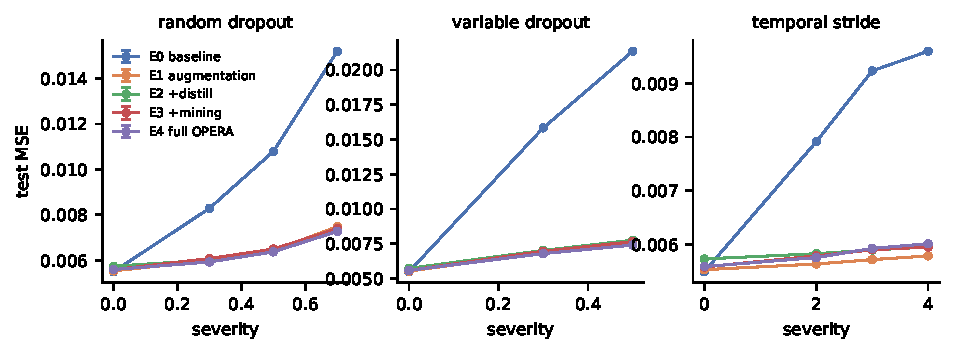
\includegraphics[width=\linewidth]{figures/fig3_robustness_curve.pdf}
\caption{Error against observation-process severity on PhysioNet\prelim, for three process families. Severity $0$
is the dataset's own observation process. Without any mechanism (blue) error grows steeply in every family; every
configuration trained with observation-process augmentation stays close to its clean error, including for stride
subsampling, a family absent from the training pool.}
\label{fig:curve}
\end{figure}

\begin{table}[t]
\caption{Mechanism isolation on PhysioNet (test MSE\prelim). ``pool'' is the hard-mining candidate pool of
Section~\ref{sec:splits}. Read $\Delta$ beside the absolute columns, not instead of them.}
\label{tab:components}
\small
\begin{tabular}{lrrrr}
\toprule
configuration & clean & mean shift & worst & $\Delta_{\mathrm{shift}}$ \\
\midrule
no mechanism & \textbf{0.00549} & 0.01137 & 0.02134 & $+107.0\%$ \\
augmentation & 0.00553 & 0.00632 & 0.00772 & $+14.3\%$ \\
\quad $+$ distillation & 0.00573 & 0.00644 & 0.00776 & $+12.3\%$ \\
\quad $+$ mining, pool $=P_{\mathrm{mix}}$ & 0.00558 & 0.00641 & 0.00765 & $+14.8\%$ \\
\quad $+$ mining, harsher pool & 0.00562 & \textbf{0.00626} & \textbf{0.00721} & $+11.4\%$ \\
all three, pool $=P_{\mathrm{mix}}$ & 0.00559 & 0.00632 & 0.00741 & $+13.1\%$ \\
all three, harsher pool & 0.00590 & 0.00653 & 0.00748 & $\mathbf{+10.7\%}$ \\
\bottomrule
\end{tabular}
\end{table}
